\section {議論}
\label {sec: discussion}

\subsection {平方根だけなの}

本稿では議論を簡素化するために,ごく単純な例題として平方根を計算する例を用いた.この例の直接の発展として,\verb|NewtonRaphson|に$x^k - a$を与える$k$-乗根の計算や,条件次第ではより収束の速いと言われる式についての適用を行った.

この研究のきっかけはC++で記述されていたSNSの可視的解析システムのPythonへの移植にある.Pythonは統計処理,グラフ処理,機械学習の豊富なライブラリを備えており,高速グラフィックスのためのOpenGLのライブラリも提供していたのだが,3次元グラフィックスに必要な空間変換のライブラリで適切なものがなかったため自作することとした.

この作業において,RiccioのOpenGL Mathematics (GLM, C++, \cite{creation--opengl-mathematics}),Gohlkeのtransformations.py (Python, \cite{gohlke--transformations.py}),Brettのtransforms3d (Python, \cite{brett--transforms3d})を参考にした.ここでtransforms3dはGolkeの協力のものtransformations.pyを発展させたものである.興味深いことにBrettが書いたREADMEには以下の記述がある.

\begin {quote}
We have tried to document the algorithms carefully and write clear code in the
hope that this code can be a teaching reference.  We document the math behind
some of the algorithms using `sympy' in ``transforms3d/derivations''.
\end {quote}

たしかにBrettのコードは読み易く,内部で用いられているアルゴリズムについては引用元となる書籍やウェブサイトへの参照が提供されている点で普通のAPIに比べて優れている.しかし,ここから生成されるAPIドキュメントをひとつの書物として見る場合は,その完全性が乏しいと言わざるを得ない.問題はBrettの手になるtransforms3dのAPIドキュメントの欠陥ではなく,おそらく世の中にあるほとんどの3Dグラフィックスライブラリの状況がこのレベルにすら達していないことである.

われわれは今回の提案を3次元グラフィックスのための空間変換ライブラリAPI(四元数,拡大縮小変換,回転変換,平行移動変換,モデルビュー変換,LookAt変換,正射影,透視投影変換など)の構築に応用した.詳細は省くが\ref {fig: t3d}図は,そのうちLookAt変換行列を生成する機能について生成したドキュメントの一部である.このプロジェクトにおいては,線形代数における方程式系の解と線形代数演算を利用することでプログラムコードとドキュメントコードの簡素化に成功している.

\begin {figure}
  \rule {\linewidth}{1pt}
  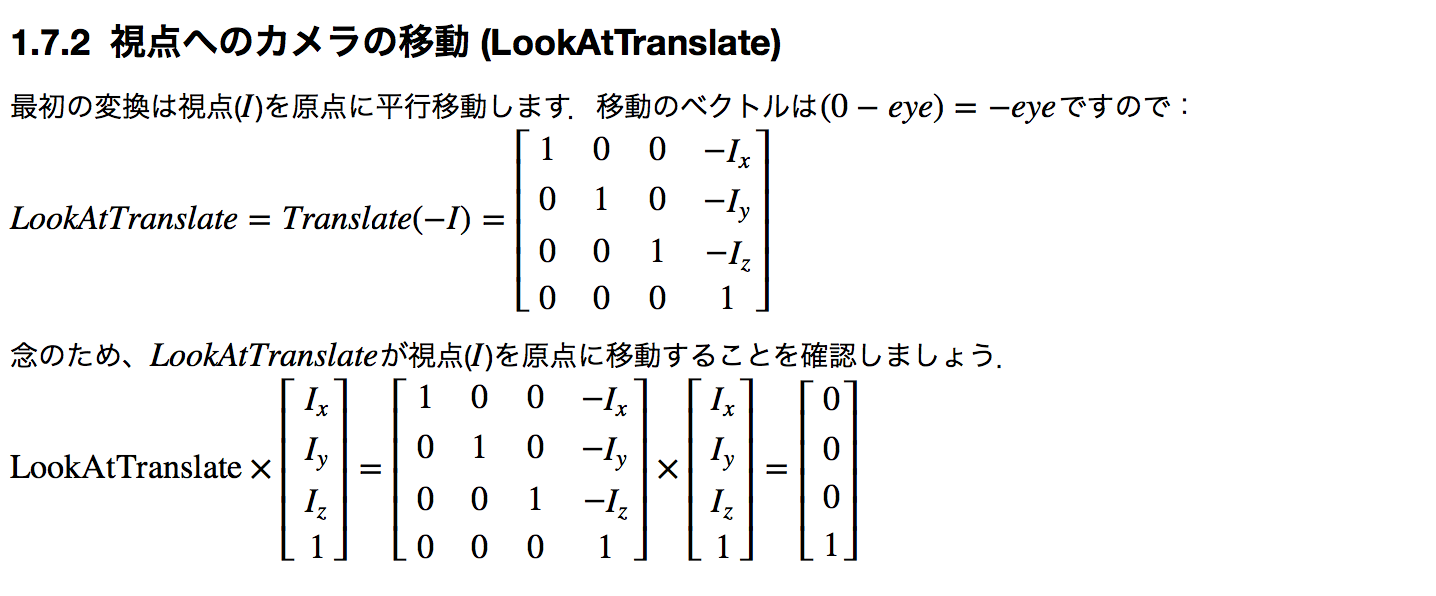
\includegraphics [width=\linewidth] {lookat-prologue.png}
  \centerline {\textbf {中略}}
  \medskip
  
  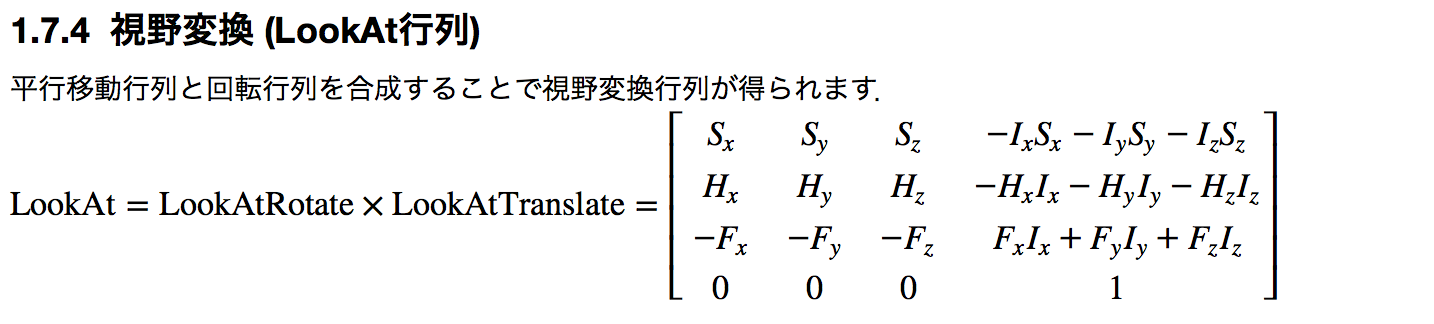
\includegraphics [width=\linewidth] {lookat-epilogue.png}\\
  \rule {\linewidth}{1pt}

  \caption {本稿の技術を応用して生成された3次元グラフィックスライブラリのAPIドキュメントより,LookAt変換のドキュメント.}
  \label {fig: t3d}
\end {figure}

本稿で提案した技術は,いくつかの対話的なグラフ構造の可視化システムの構築に応用されている.武田は無向グラフを力学的モデルによって可視化する基本的なアルゴリズムの記述にSymPyを用いた\cite {takeda-2016-sympy-kk}.このアルゴリズムでは,グラフの頂点間に仮想的にバネを張り巡らし,それらのバネ群が構成するポテンシャルエネルギーを最小化することでグラフを定める.\cite{kamada-1991-a-general-framework-for-visualizing-abstract-objects}この研究では,ポテンシャル関数をSymPyで記述した上で,その一次微分と二次微分を数式として得たものをlambdifyによってPythonの関数を得ている.二次微分で得られるヘッセ行列は巨大であり,人手でこれを正確に計算し,そのとおりのプログラムを作成することには困難を伴なう.

高野は対話的な高次元グラフ可視化システムであるAGI3Dのアルゴリズム\cite{wakita-2015-interactive-high-dimensional-visualization-of-social-graphs}の記述を試みた\cite {takano-2016-sympy-agi}.AGI3Dのアルゴリズムでは,マウスドラッグ操作を高次元回転操作に翻訳する過程で制約充足問題を解いている.この研究では,比較的簡単な制約式から思いがけず複雑な制約設定系を半自動生成することで,200行ほどの難解なプログラムコードを数十行の数式処理に変換している.これらの数式処理の記述は,このアルゴリズムの背景となっている統計理論と対応しており,理解も容易になった.

これらの記述例は限定的ではあるものの,微積分,線形代数,物理シミュレーション,大規模行列などという比較的広い数学領域を覆っている.以上の結果より,本稿で提案しているアプローチが数学や物理の広い分野の問題の記述に利用できるという感触が得られた.

\subsection {ほかの領域への応用}

\begin {figure}

  \begin {subfigure}{.99\linewidth}
    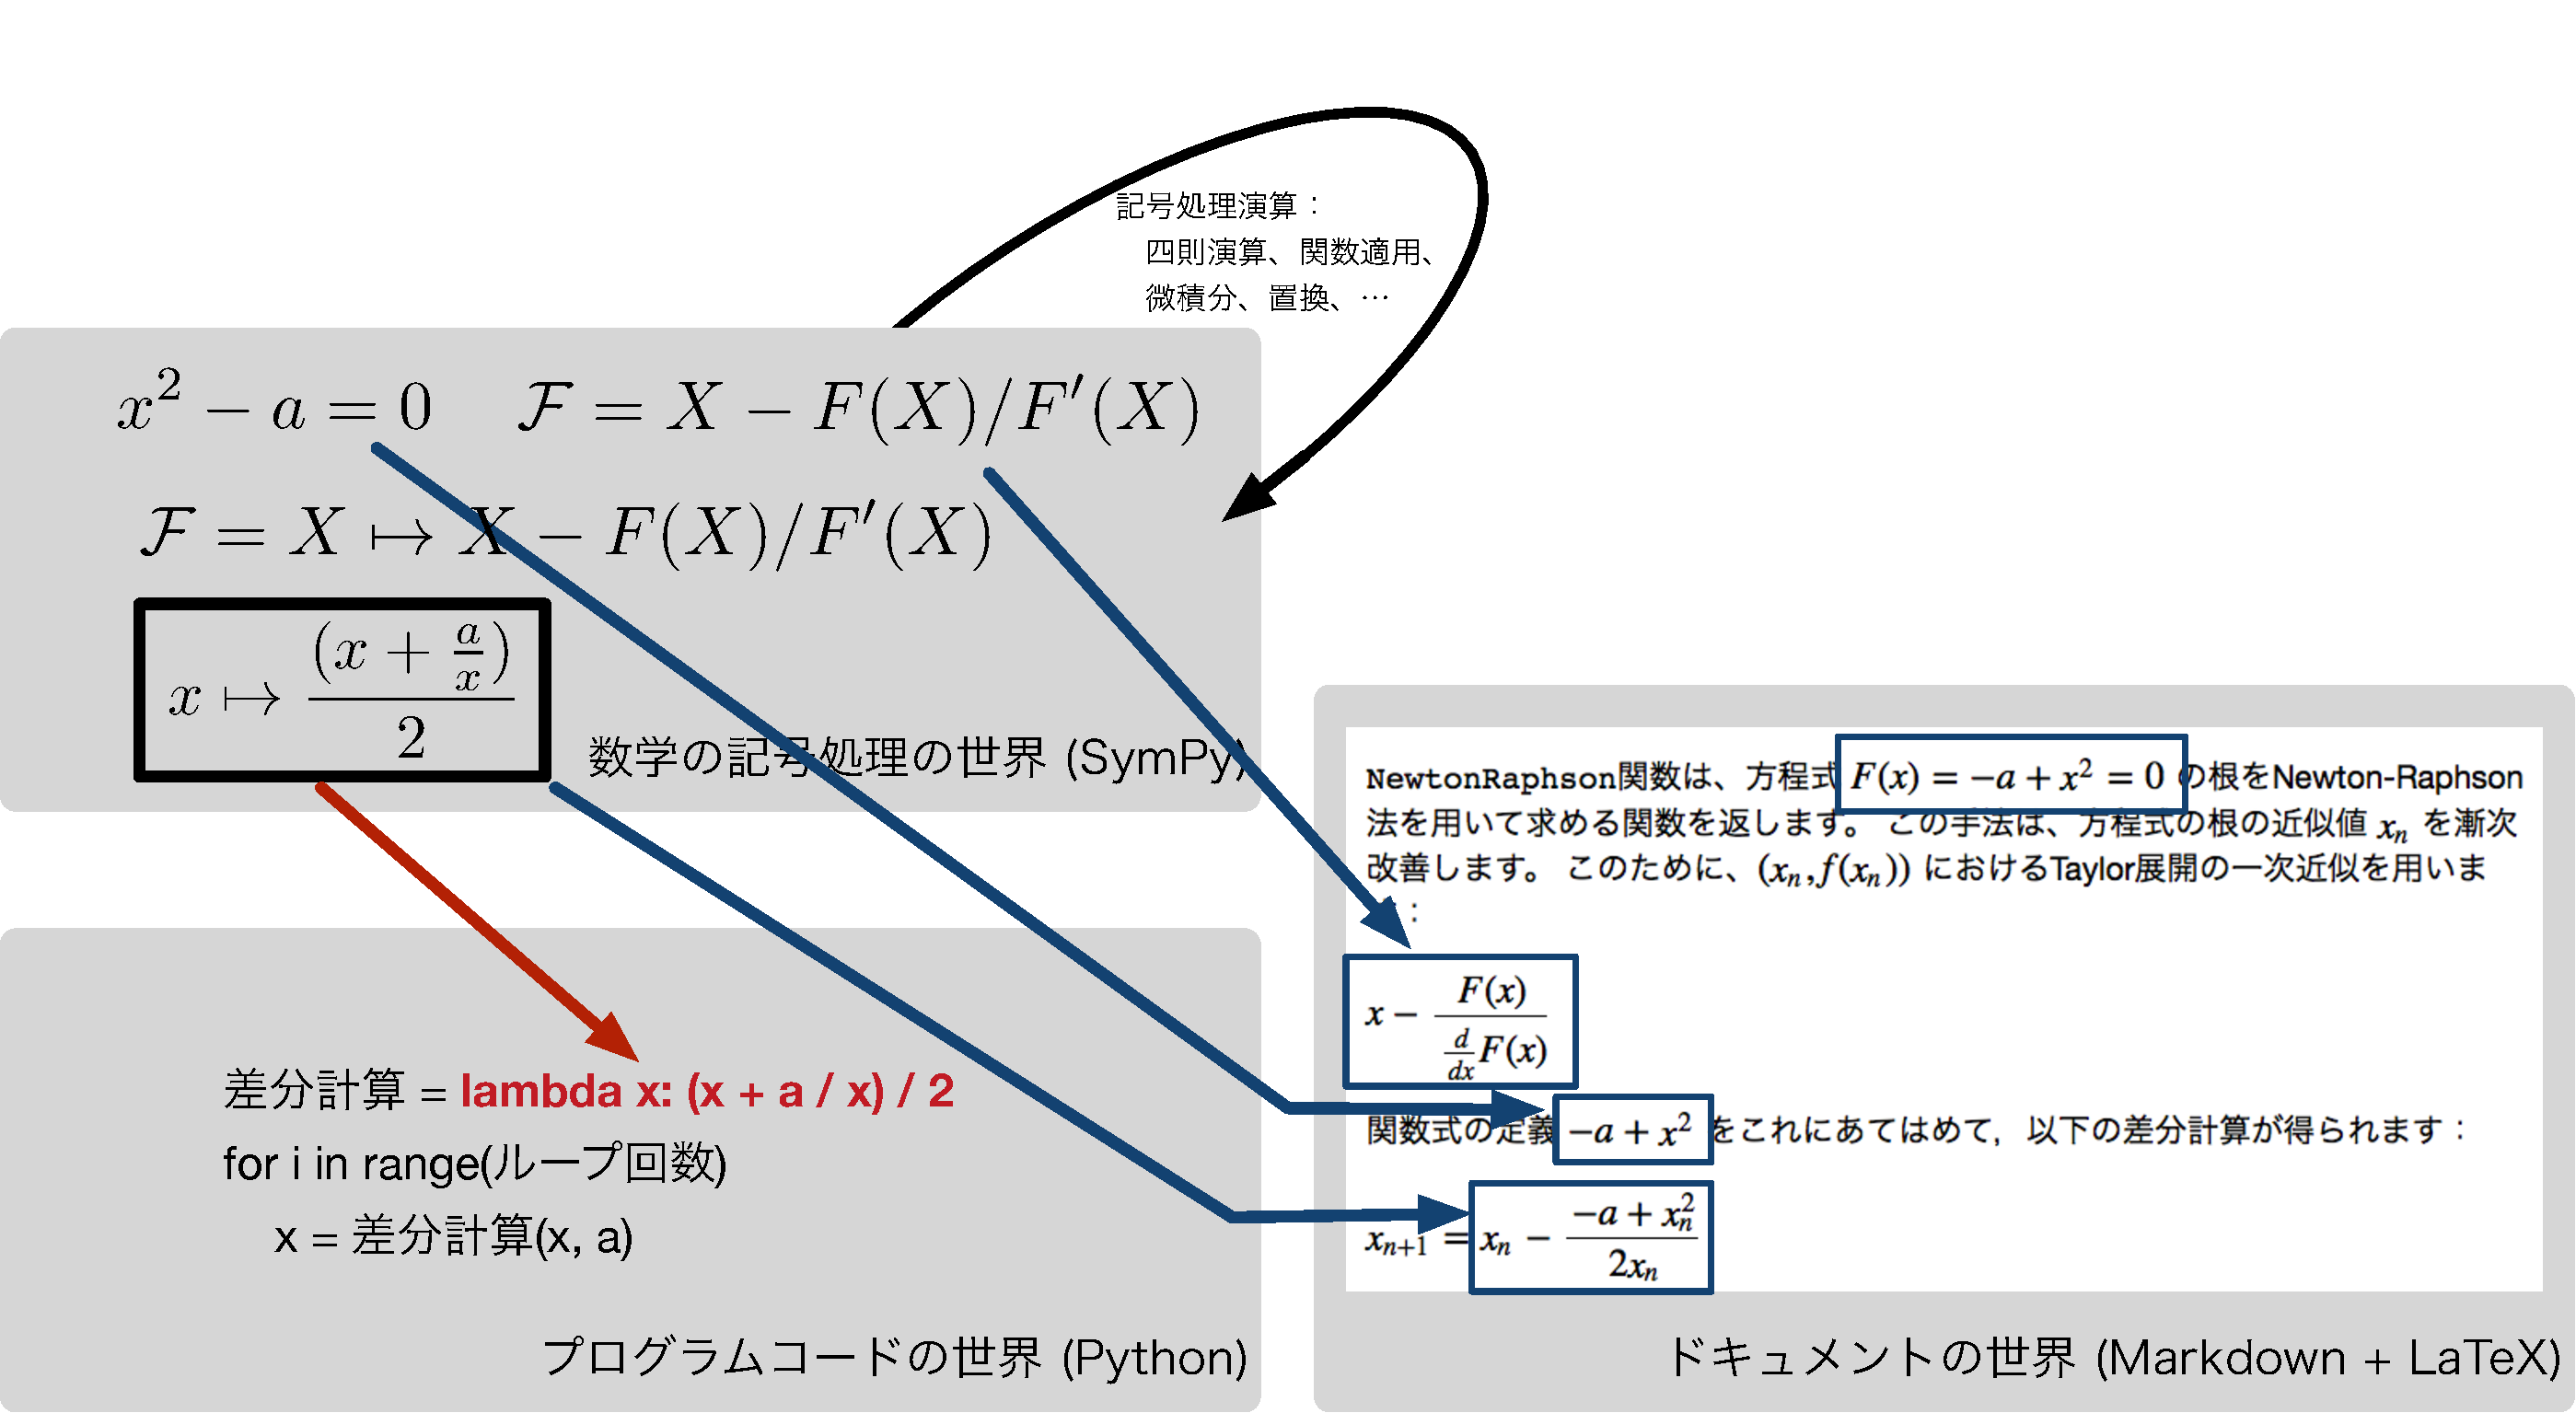
\includegraphics [width=\linewidth] {sympy-outline.pdf}
    \subcaption {本稿の提案のアウトライン}
    \label {fig: sympy outline}
  \end {subfigure}

  \begin {subfigure}{.99\linewidth}
    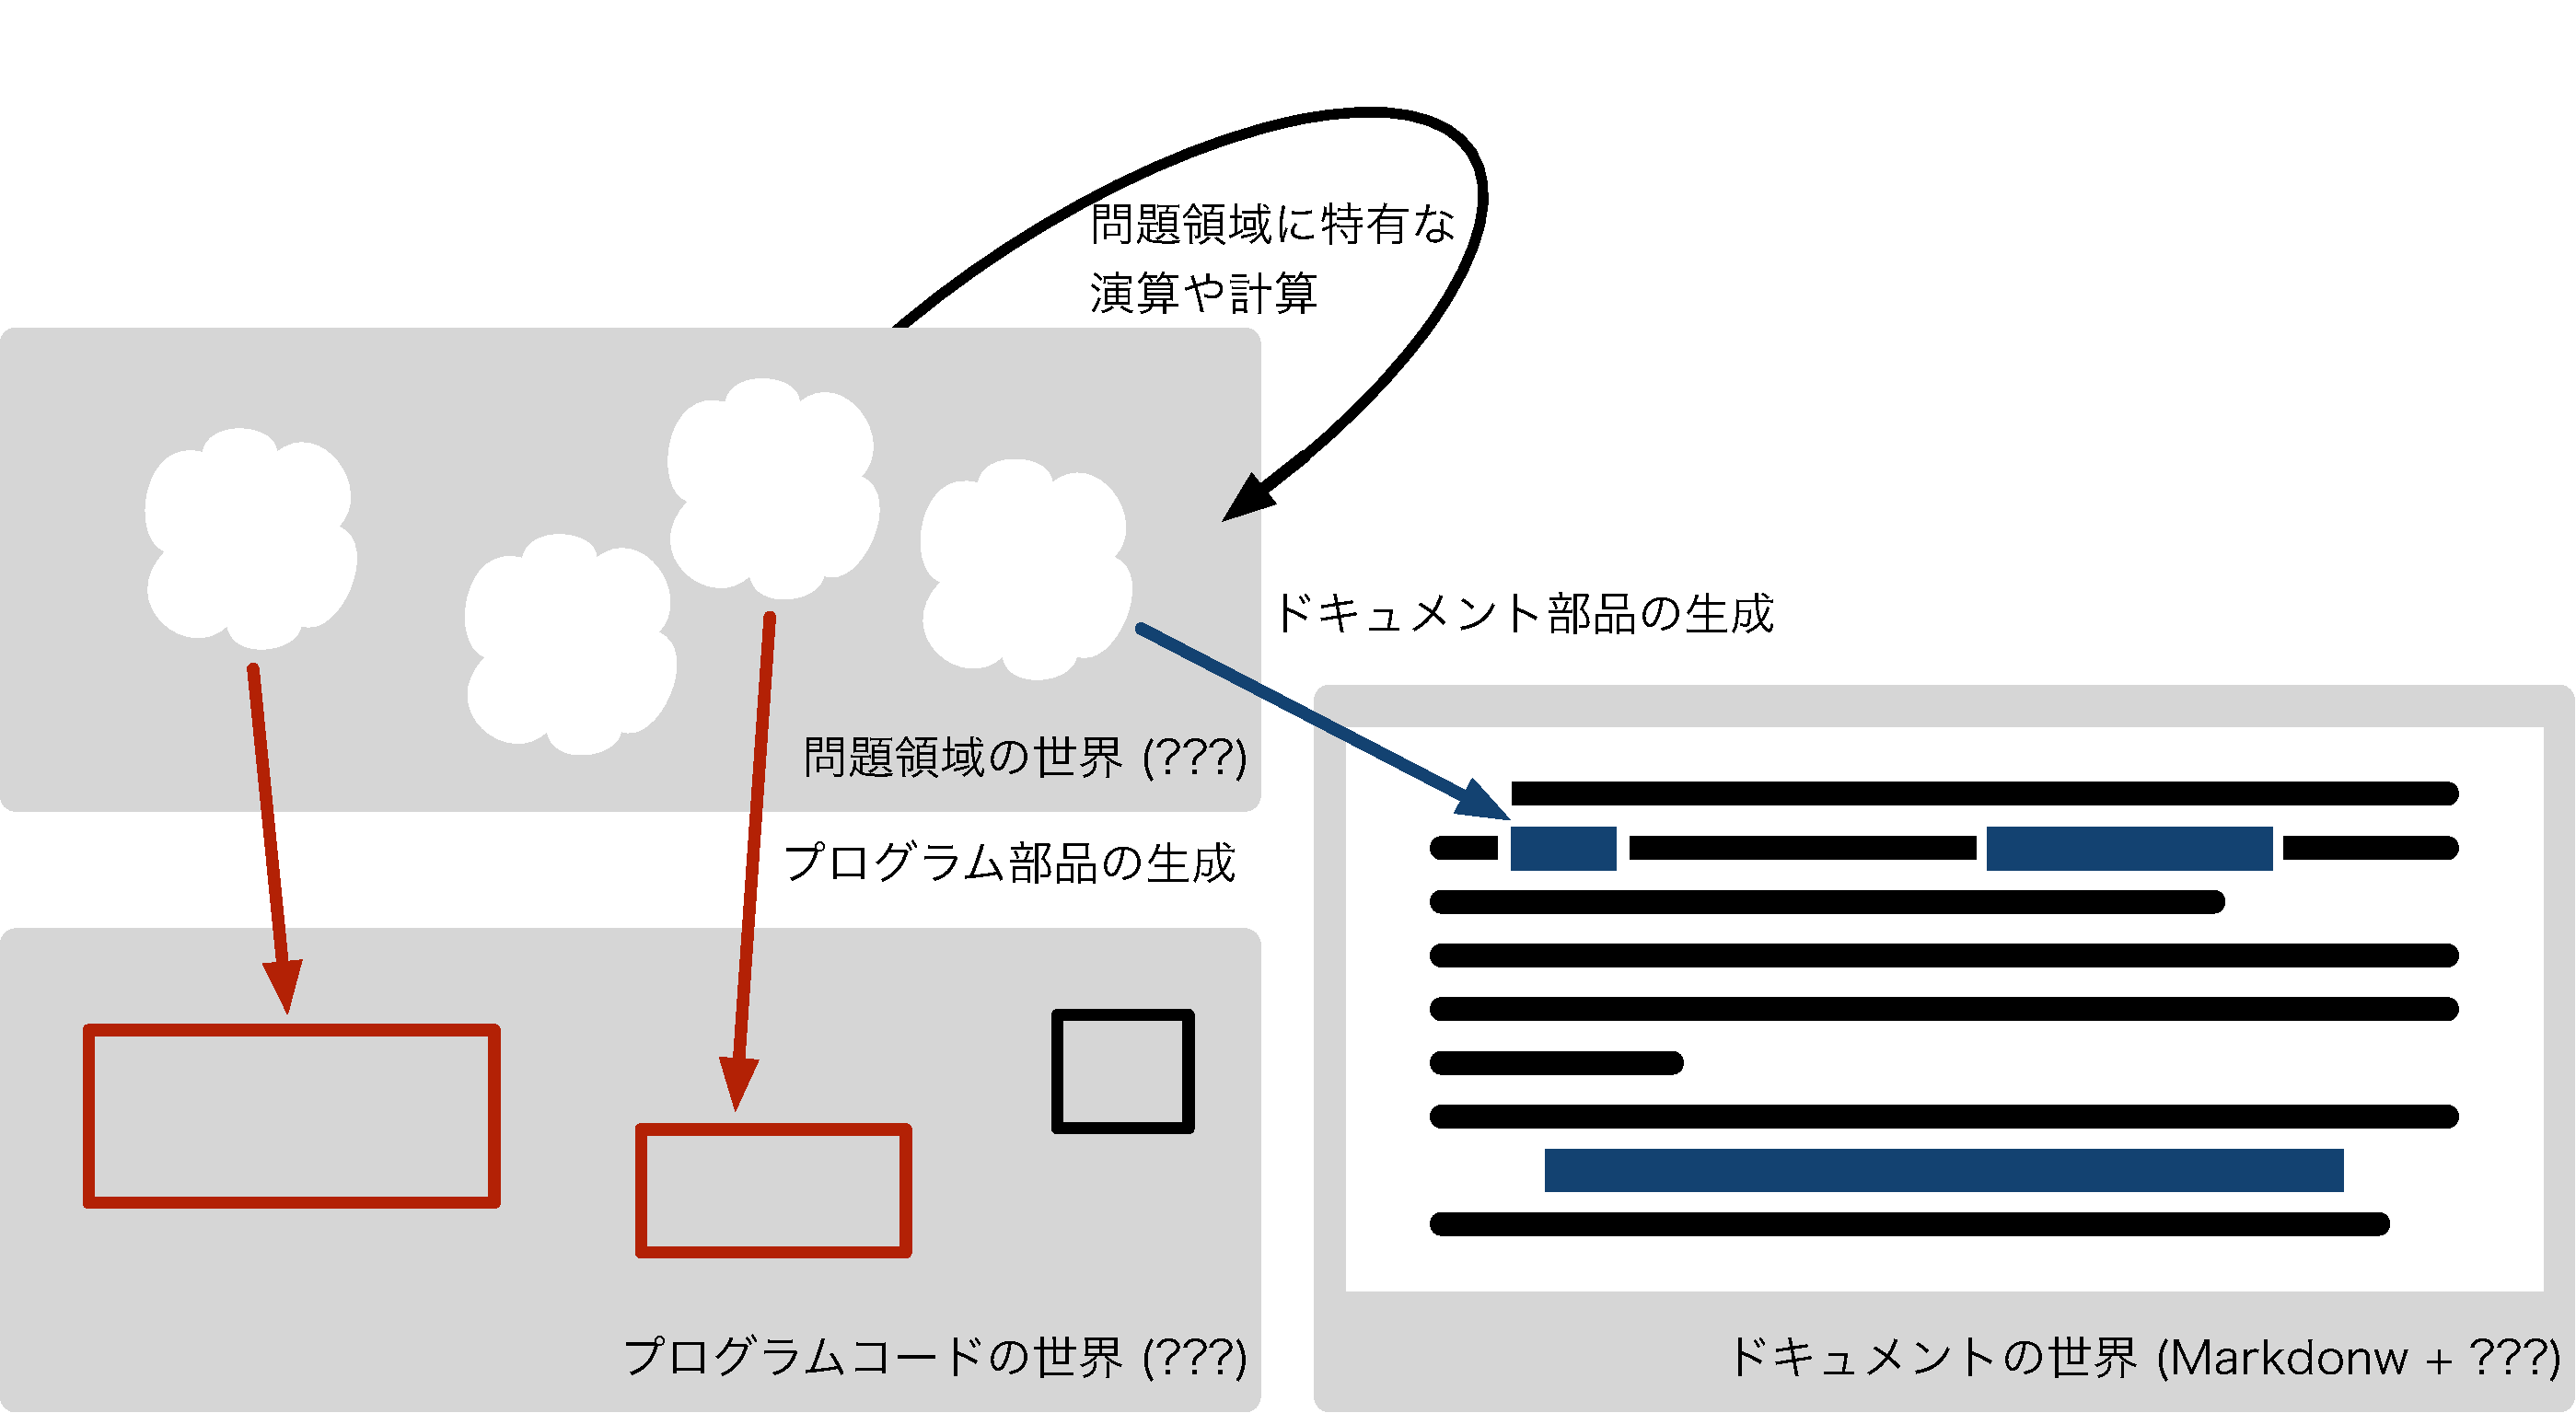
\includegraphics [width=\linewidth] {general-outline.pdf}
    \subcaption {数学的知識を問題領域とした本稿の提案を抽象化し,他の問題領域への適用を検討すると...}
    \label {fig: general outline}
  \end {subfigure}

  \caption {より広い問題領域への応用をめざして}
  \label {fig: outline}

\end {figure}

本稿では数学的知識を背景とするソフトウェアにおけるプログラム作成とドキュメント執筆について問題を明らかにするとともに数式処理システムを利用したエレガントな解決策を提示した.この仕組みを模式的に表現したものが図\ref {fig: outline}\subref {fig: sympy outline}である.

ここで扱っている問題は3種の世界,すなわち問題領域を自然に記述可能な\emph {数学の世界},計算として実行するための\emph {プログラムの世界},さらにプログラムを理解するための用意する\emph {ドキュメントの世界}があること,それらの間に実は密接な関係があるのだが,これまでほとんどの場合,それを人力に頼って記述していたことである.数学の世界の記述は主に数式が用いられ,プログラミングの世界ではプログラミング言語が利用され,ドキュメントの世界ではプログラムコメント,ワープロ,表計算ソフト,マークアップ言語などが利用されてきた.ソフトウェア技術者たちはこれらのツールを場当たり的に活用してドキュメントを用意してきた.

これに対して,本稿の提案では数式処理システムSymPyを用いることで,数学における記号処理,プログラムコード断片の生成,ドキュメントに埋め込むべき数式表現の生成を効率的に実施できた.

ところで,世の中の諸問題のなかで数学的知識を背景とするものはわずかである.そのほかの問題についてはどのようにアプローチすべきだろう.

それぞれの領域ごとに問題となっている概念を記述する記述系というものがある.たとえば,音楽でいえば楽譜であったり,音楽演奏でいえばMidiデータである.法律でいえば,法律の条文や判例がそれにあたるだろう.

今回の数式処理システムは幸運な例であり,数式という領域を形式的に記述するための枠組みがSymPyライブラリの実装として備わっていた.また,SymPyが提供するコード生成系とLaTeX風の数式生成系を利用することにより,数学の世界からプログラミングの世界,そしてドキュメントの世界への橋渡しの用意があった.実際,本稿のプロジェクトを実施する上で著者らが追加した仕掛けは,図\ref {fig: md function}に掲げたもの程度にすぎない.

一方,このほかの領域において,これだけの仕掛けが完備している例は少ないかもしれない.そもそも,数学ほど形式的な理解が進んでいない領域も多いだろうし,Midiデータのようにデジタル化はされているものの,それを問題領域における音楽の理解として把握することにはまだもう少し準備が足りないように思えるものもある.ほとんどの領域では不定形,あるいは場当たり的で煩雑な知識の記述が用いられているのではないだろうか.

本稿での成果を他の領域へ展開するにあたって,最初の障害がその領域の知識を形式的に記述することである.幸運なことにわずかな努力でそれが達成できる領域が存在した場合は,形式化されたその領域の知識から,望ましい計算を取り出すための\verb|lambdify|のような関数を提供するとともに,一般的な文書に組込むための変換器を用意すればよいように思う.図\ref {fig: outline}\subref {fig: general outline}は,この議論を模式的に表したものである.言うは易き行うは難しではあるが,この図を念頭にすこしでも応用範囲を広げられないか考察を深めたい.

\subsection {数式的テストケース}

\begin {figure}
  \rule {\linewidth} {1pt}
  \bgroup \small \color {darkred}
  \verbatiminput {code/symbolic-test.py} \egroup

  \caption {数式的テストケースの例}
  \label {fig: symbolic test}
  \rule {\linewidth} {1pt}
\end {figure}

SymPyは数式を簡約するための\verb|simplify|関数を提供している.これを利用することで二つの数式の等価性を判定できる場合がある.たとえば,ふたつの実数値をとる数式\verb|e1|と\verb|e2|に対して,\verb|e1 == e2|によって,等価性について判断できる場合がある.\footnote {もちろん任意の数式の組について等価性を判定できるわけではない.}

図\ref {fig: symbolic test}はこの性質を利用し,視野錐台が透視投影変換によって単位立方体に射影されることを確認している.ふたつの数式の恒等性は,数式に出現する記号への任意の値の割り当てについての恒等性を意味する.このため,変数への割り当てについての有限のサンプルについて等価性を確認する通常の単体テストよりも強力な道具立てとなる.

\subsection {なぜSymPy,なぜPython}

数式処理システムとしてのSymPyは一定の有用性はあるものの,まだまだ基本的な機能で欠けているものもあり,バグも多い.数式処理システムとしての能力としてはMapleやMathematicaの方がはるかに高機能で安定しているだろう.

本研究でSymPyを用いた理由は,たまたまPythonを用いた開発のなかで問題を発見をしたことにすぎない.しかし,PythonのためのPythonライブラリとして提供されている数式システムというSymPyは面白い位置付けにある.まず,SymPyは言語ではなく拡張ライブラリであるため,Pythonのアプリケーションと統合して利用することが用意である.また,数式を実装する計算をPythonが提供する無名関数(\verb|lambda|)として提供しているため,アプリケーションの実行時に数式処理を施して,その場で処理された数式に関する数値計算ができることも魅力的である.もしも,SymPyがライブラリでなく(MapleやMathematicaのような)独自の数式処理言語だったら,あるいは,数式から計算への変換に無名関数を用いていなかったら,オフラインでコード生成とリンク作業が必要になっていたことであろう.

ところで,数式から実行可能なコードを出力する機能はSymPyの専売特許ではない.MathematicaはC言語のコードを生成することができ,MapleはC, Fortran, JavaScript, Pythonを始めとする多くのプログラミング言語のコードを生成できる.一方,SymPyは本稿で紹介したPython lambdaの生成だけでなく,C, Fortran 95, JavaScriptといった汎用プログラミング言語とOpenCLやCUDAのような汎用GPU計算もサポートしている.

いくつかの数式処理システムとそれらが提供するコード生成器を利用すれば,本稿と同様の試みに近いことはできるかもしれない.ただ,本研究の成果が比較的容易に得られた背景として,Jupyter Notebookの存在は無視できない.\footnote {Jupyter Notebookの前身であるiPython環境\cite{perez-2007-ipython-a-system-for-interactive-scientific-computing}は,Mathematica Notebookに触発されて開発されたPython用のノートブック環境であった.iPythonのノートブック機能を多言語化して多くのインタプリタ言語に対応させたものがJupyter Notebookである.\cite{jupyter-2016-notebooks}}HTML, Markdown, MathJaxを併用できるノートブックの存在がなかったならば,本稿のアイデアもさまざまな変換器を組み合わせた,実用性が疑わしいものとなっていただろう.そもそも,著者らも,このような研究を始める気にすらならなかったかもしれない.Jupyter Notebookの存在は本研究の成果において重要であった.

本稿のアイデアに基づいて,類似した試みをするために,いくつかの数式処理システムとさまざまなプログラミング言語を利用することが考えられるが,数式処理,プログラムの作成,ドキュメントの執筆という3つの作業を滑らかに実施するための,もっとも素直な環境はJupyter Notebook for Python基盤の上でのSymPyの利用であろうと思われる.
